\section{MLP architecture}
The MLP model architecture for the classification task can be visualized in Table \ref{tab:mlp_str}.
\begin{table}[!h]
    \centering
    \begin{tabular}{|c|c|}
    \hline
    Layer(type)&Output shape  \\
    \hline\hline
    Embedding&(None,74,32)\\
    \hline
    Flatten&(None,2368)\\
    \hline
    Dense&(None,250)\\
    \hline
    Dense&(None,1)\\
    \hline
    \end{tabular}
    \caption{MLP architecture diagram}
    \label{tab:mlp_str}
\end{table}

\section{Receiver Operating Characteristic curve}
According to the given metric of each model, we can plot the ROC curve. By observing the curve of each plot, both models have almost the same curvature in the beginning of the curve. Every curve tends to have an dramatic increase in ROC curve between 0 and 0.1. The Area Under Curve and the curve of the plot 
support the claim that the SVM classifier is the best among our compared models, irrespective of the chosen metric of comparison.

\begin{figure}[H]
\centering
\minipage{0.4\textwidth}
  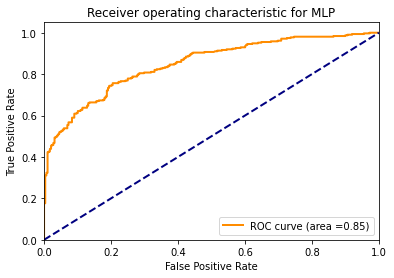
\includegraphics[width=\linewidth]{Images/mlp_roc.png}
  \caption{ROC - MLP}\label{fig:awesome_image1}
\endminipage\hfill
\minipage{0.4\textwidth}
  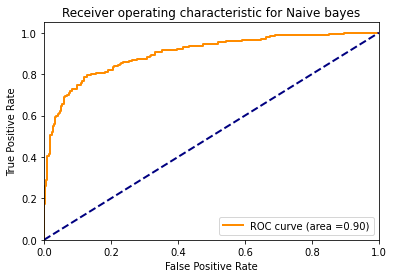
\includegraphics[width=\linewidth]{Images/nb_roc.png}
  \caption{ROC - Naïve Bayes}\label{fig:awesome_image2}
\endminipage\hfill
\minipage{0.4\textwidth}%
  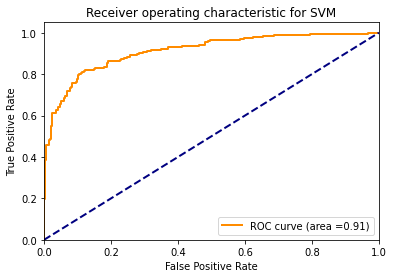
\includegraphics[width=\linewidth]{Images/svm_roc.png}
  \caption{ROC - SVM}\label{fig:awesome_image3}
\endminipage
\end{figure}

\section{Keyword generation - qualitative analysis}\label{cloudwords}
One of the visualizations options that can be exploited for a further qualitative analysis is the word-cloud technique. Figures \ref{fig:pos} and \ref{fig:neg} exemplify the results obtained using the YAKE text mining algorithm and our proposed generation model.
\begin{figure}[H]
  \centering
  \minipage{\textwidth}
  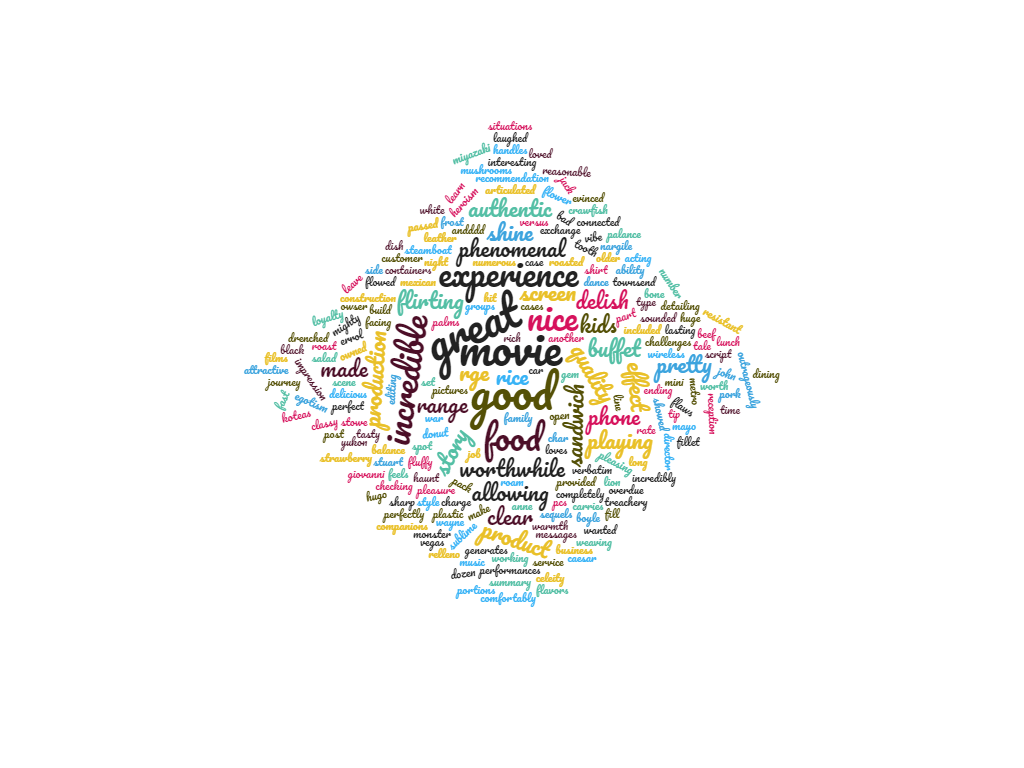
\includegraphics[width=\linewidth]{Images/yake_pos.png}
  \caption{YAKE - positive}
  \label{fig:pos}
\endminipage\hfill
  \minipage{\textwidth}
  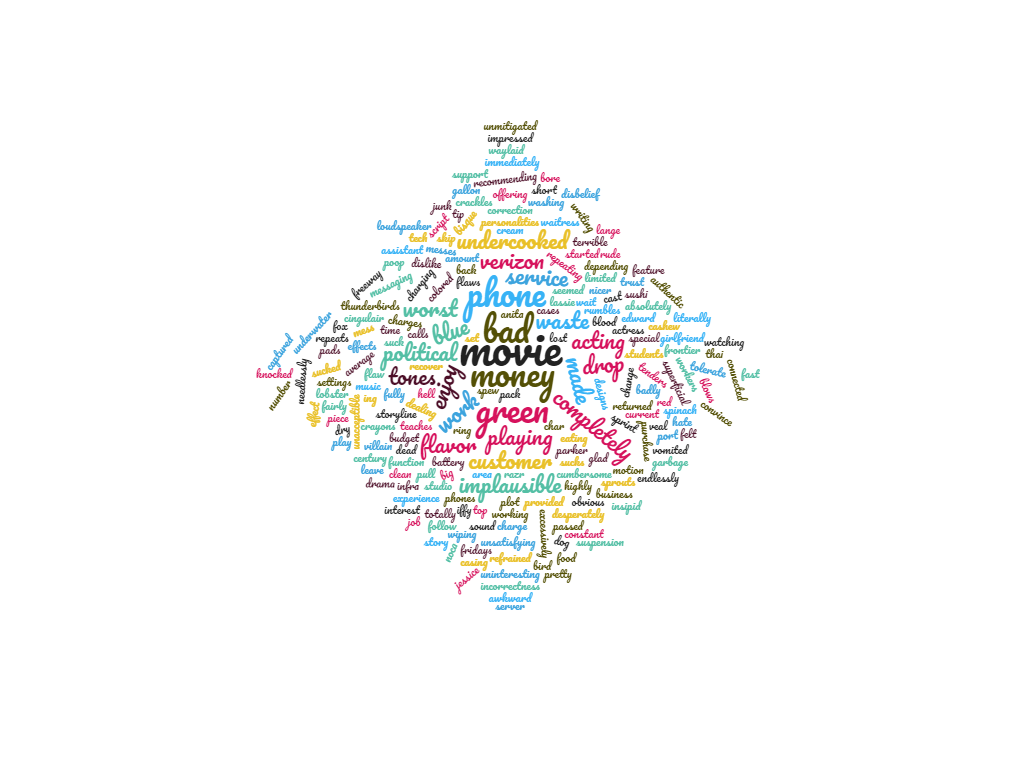
\includegraphics[width=\linewidth]{Images/yake_neg.png}
  \caption{YAKE - negative}
  \label{fig:neg}
\endminipage\hfill
\end{figure}%
